
%%% Local Variables:
%%% mode: latex
%%% TeX-master: t
%%% End:

\chapter{PARD原型系统}
\label{chap:impl}

基于前四章的设计,本文实现了资源管理可编程体系结构PARD的原型系统,
包括基于gem5的全系统模拟器实现以及Xilinx VC709平台上的FPGA原型。
之前的章节中已经通过模拟器对PARD体系结构的部分功能进行了验证,
本章将着重介绍FPGA原型系统的设计与实现,包括:
基础系统选择与原型系统架构、PRM软件栈实现、以及控制平面与数据平面实现。
最后对FPGA原型系统的功能以及开销进行分析。


\section{FPGA原型系统}

模拟器在体系结构研究中有着不可或缺的作用,但它也有十分明显的缺点,
即模拟速度过慢,性能无法支持真实应用的运行。
PARD模拟器也面临这样的问题:
使用该模拟器运行典型的数据中心应用memcached,
其3秒的执行需要超过30个小时的模拟时间。
这使得该平台只能作为本文技术点验证的工具,
而全系统的功能验证,需要一个性能更高的实验平台。
基于以上动机,本文同时实现了PARD体系结构的FPGA原型系统,
用于全系统功能的验证,并对系统资源开销的精确评估。

\subsection{基础系统选择}

实现PARD原型系统的第一个工作是选择一个合适的基础系统,
PARD对基础系统有以下需求:

\begin{enumerate}[leftmargin=2\parindent, nolistsep, label=\arabic*)]
  \item 能够在FPGA环境下综合;
  \item 独立系统,不依靠任何辅助设施即可运行;
  \item 丰富的I/O设备支持,支持Xilinx VC709开发板所提供的外设,如以太网和PCI-Express;
  \item 能够运行Linux操作系统;
  \item 频率/性能足够运行常见Benchmark应用,如SPECCPU、PARSEC等;
  \item 可以运行典型的数据中心应用,如memcached、httpd等;
  \item 具备完整的软件开发环境;
\end{enumerate}

虽然在开源领域有大量可用的处理器软核,如Oracle OpenSPARC T1\cite{opensparct1}、
RISC-V\cite{riscv}、OpenRISC\cite{or1k}、LEON3\cite{leon3}等,
但这些软核并不能满足PARD原型系统的需求。
其中OpenSPARC T1和RISC-V目前的FPGA实现并不是一个独立系统,
需要额外的处理器(如MicroBlaze或ARM)作代理以实现访存与I/O操作;
OpenRISC 1200的软件开发环境支持并不完整;
LEON3是目前开源的处理器软核中最为合适的选择,但其对linux内核的支持并不好,
目前只能运行早期的内核版本,同时软件环境也比较老旧,运行数据中心应用存在一定的困难。
一些FPGA厂商也提供了可配置的处理器核,
如Xilinx的MicroBlaze\cite{microblaze}和ARM\cite{zynq},以及Altera的NIOS II\cite{niosii}。

本文最终选择了Xilinx的MicroBlaze作为基础系统,
其处理器采用32位小端RISC架构,实现了单发射5级流水,
支持MMU及虚拟内存,使用AXI4作为外部总线接口\cite{microblaze-ref}。
该处理器软核在Virtex-7型号的FPGA上频率最高能够达到246MHz,
性能是354DMIPs(1.44DMIPs/MHz)\cite{microblaze},能够满足PARD原型系统的需求。

\begin{figure}[tb]
  \centering
  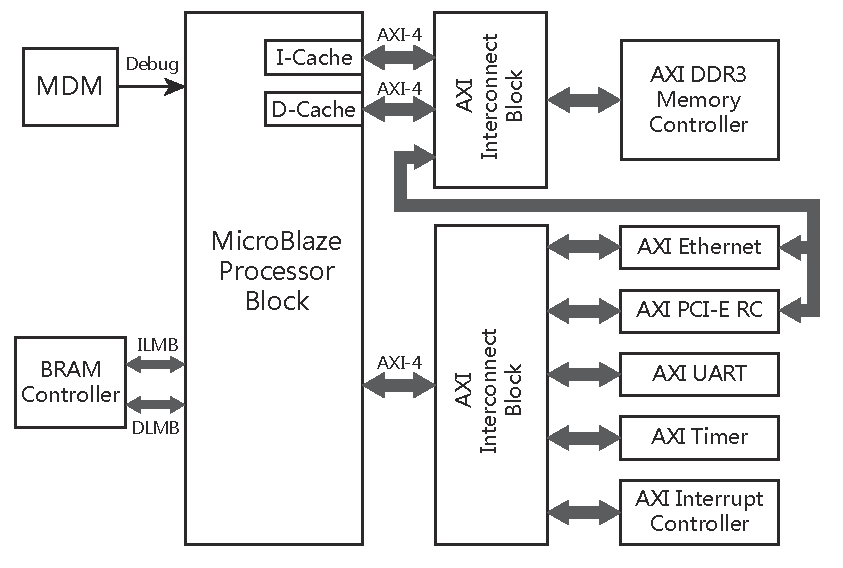
\includegraphics[width=0.6\textwidth]{impl/microblaze-base-arch}
  \caption{MicroBlaze基础架构}
  \label{fig:microblaze-base-arch}
\end{figure}


基于MicroBlaze的一个典型系统架构如图\ref{fig:microblaze-base-arch}所示,
MicroBlaze系统的固件代码保存在Block Memory中,
通过LMB(Local Memory Bus)总线连接到处理器核;
缓存子系统采用哈佛结构,具有分离的指令与数据缓存,它们通过AXI4总线连接到内存控制器;
I/O子系统同样使用AXI4总线互连,其中包括基本的外设,如中断控制器、串口、时钟等,
也支持一些复杂的I/O设备,如以太网\cite{axi-ethernet-subsystem}、
PCI-E\cite{axi-pcie-bridge}等。
MicroBlaze同时还提供了硬件调试接口,可以通过JTAG对其进行调试。

目前Xilinx提供的MicroBlaze软核并不支持多处理器架构,
在硬件实现上没有提供处理器间同步、通信机制,
之前一些工作\cite{microblaze-mp-rsp08,microblaze-mp-xapp}尝试为其增加多处理器支持,
但这些工作只是实现也最底层的处理器间同步、通信机制,
没有可用的操作系统层次上的多核支持。
受到该因素的影响,本文所设计的PARD原型系统只实现了``伪多核''的系统,
即系统中存在多个处理器核,但每个一逻辑域都被限制为只能使用一个处理器核。
未来MicroBlaze的多核软硬件支持完善后,可以很容易的将PARD原型系统的这一限制解除,
实现真正的多核系统。


\subsection{PARD原型系统架构}

PARD原型系统架构如图\ref{fig:pard-arch-impl}所示,
该系统由处理器子系统、I/O子系统、PRM SoC三部分组成。
其中处理器子系统包含4个处理器核心、共享缓存和内存控制器;
I/O子系统中包含4个串口控制器、2个以太网控制器和1个PCI Express根逻辑(RootComplex),
系统中所有的数据通路使用AXI4总线连接;
PRM同样是基于MicroBlaze的SoC系统,对外提供串口与SFP以太网接口,
同时通过内部串口与I/O子系统相连,用于接收I/O子系统的串口输出,
使用$I^2C$总线作为控制平面网络的数据链路层,通过$I^2C Switch$连接到系统中的4个控制平面:
处理器核控制平面CoreCP、共享缓存控制平面CacheCP、内存控制器控制平面MemCP和
I/O子系统控制平面I/OCP。

\begin{figure}[tb]
  \centering
  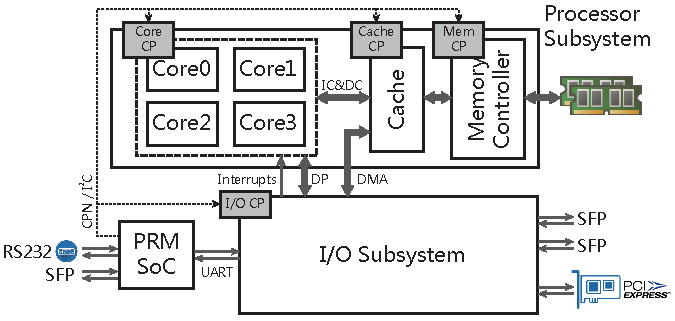
\includegraphics[width=0.8\textwidth]{impl/pard-arch-impl}
  \caption{PARD原型系统架构}
  \label{fig:pard-arch-impl}
\end{figure}

% 如何增加标签寄存器
处理器核心使用MicroBlaze软核及其他附属模块组成,
其内部结构如图\ref{fig:pard-core-impl}所示,
其中包含MicroBlaze软核、中断控制器和时钟模块,
该模块从外部输入时钟、复位和中断信号,
通过3个AXI4接口(IC指令缓存端口、DC数据缓存端口和DP外设端口)与外部交换数据。
AXI4总线协议中使用独立的通道实现读写请求、数据与响应,
其中读写请求中包含用户自定义信号,本文使用该信号在系统中传播应用标签。
由于MicroBlaze并没有开放源代码,处理器核的请求标记工作需要在核外进行:
首先在核外增加了一个标签寄存器,CoreCP连接到该寄存器,并可以对其内容进行修改;
在IC/DC/DP 3个端口外分别增加标签模块,
用于将标签寄存器的值附加到AXI4总线AR/AW 2个通道的USER信号中,完成请求标记。

% 增加共享缓存模块:支持16路、实现标签传播、实现划分
Xilinx为AXI4总线提供了一个缓存功能的IP核SystemCache\cite{pg118-system-cache},
其默认配置最多只能够支持4路组关联,这对于四核的PARD原型系统来说,
不足以验证缓存容量划分的功能,本文通过修改IP核实现,将其扩展到16路组关联;
按照第\ref{chap:labeladdrspace:propagation}节所述的方式,为该模块增加了标签传播功能;
同时修改其默认LRU替换策略,使其支持按路划分功能,
并通过CacheCP对共享缓存的行为进行控制。%(参见第\ref{chap:impl:cachecp}节)。
% 实现的多核
该Cache模块提供MicroBlaze专用接口连接4个处理器核,
同时还提供了通用AXI Slave接口连接I/O子系统的DMA通道。
内存控制器控制平面提供了地址映射功能,实现4个处理器核的内存资源划分。
%第\ref{chap:impl:migcp}节将详细讨论内存控制器控制平面的实现。

% I/O子系统结构
PARD的I/O子系统内部结构如图\ref{fig:pard-io-impl}所示,
处理器子系统的DP端口经过I/O子系统控制平面的地址映射后,使用AXI总线连接到所有的硬件模块,
其中PCI-E和以太网模块中包含DMA功能,
因此按照第\ref{chap:labeladdrspace:tagging}节中所描述的方法在其中增加标签寄存器,
其DMA访存请求经过标记后通过AXI总线发送到Cache模块。
所有设备的中断信号在内部进行编码,经过I/O控制平面进行重映射处理后,发送给对应的处理器核。
%I/O子系统控制平面的设计将在第\ref{chap:impl:iocp}节进行讨论。
%控制平面的实现将在第\ref{chap:impl:cp}节进行详细讨论。

\begin{figure}[tb]
\begin{minipage}{0.48\textwidth}
  \centering
  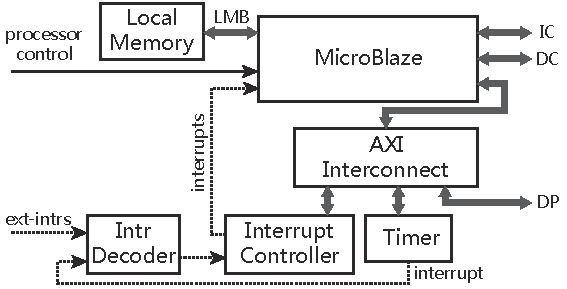
\includegraphics[width=\textwidth]{impl/pard-core-impl}
  \caption{PARD原型系统处理器核}
  \label{fig:pard-core-impl}
\end{minipage}\hfill
\begin{minipage}{0.48\textwidth}
  \centering
  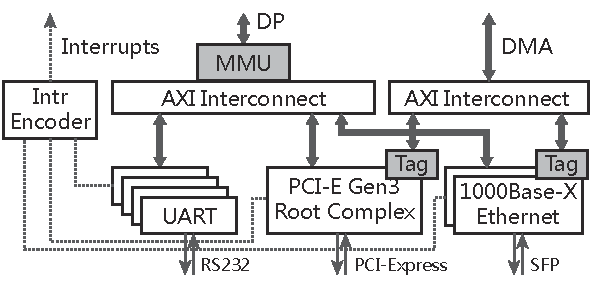
\includegraphics[width=\textwidth]{impl/pard-io-impl}
  \caption{PARD原型系统I/O子系统}
  \label{fig:pard-io-impl}
\end{minipage}
\end{figure}

% 原型的照片
本文使用Xilinx Virtex-7 FPGA(型号xc7vx690tffg1761-2)
在VC709平台上实现了上述PARD原型系统,如图\ref{fig:pard-fpga-board}所示。
该原型系统对外呈现3类接口:1个RS232串口,与PRM的串口相连;
3个SFP接口,其中2个连接到I/O子系统,另外1个与PRM的以太网接口相连;
1个PCI-E Gen3 x4接口,连接到I/O子系统,可以连接兼容的PCI-E设备,
在本例中在该接口连接了1个Intel PCI-E以太网卡(芯片型号82575)。

\begin{figure}[tb]
  \centering
  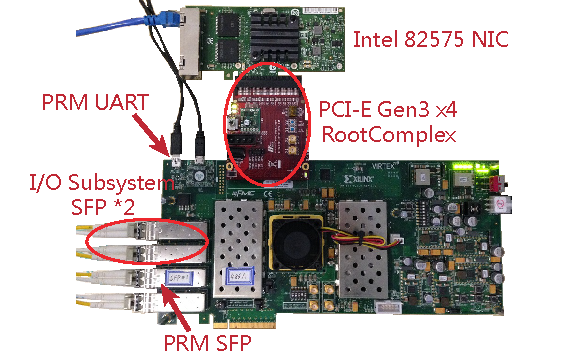
\includegraphics[width=0.6\textwidth]{impl/pard-fpga-board}
  \caption{PARD原型系统}
  \label{fig:pard-fpga-board}
\end{figure}

% 资源占用与FPGA布线结果
原型系统处理器子系统工作在133.33MHz频率,
其中内存控制器phy工作频率为400MHz,I/O子系统和PRM都工作在100MHz频率。
该原型系统在FPGA上的布局布线结果如图\ref{fig:pard-fpga-routed}所示,
资源占用方面,总计使用了49,987个Slice资源和362.5个BlockRAM资源,
分别占FPGA设备资源总量的46.16\%和24.66\%。
其中,Slice资源中有113,493个LUT用于逻辑实现,占LUT总量的26.20\%;
用作Memory(\emph{e.g.} Distributed RAM, Shift Register)的LUT共13,993个,占LUT总量的8.03\%;
Flip Flop(FF)总计使用165,707个,占FF总量的38.25\%。
布线资源使用方面,横向布线资源占用10.33\%,纵向布线资源占用8.56\%。
\textbf{TODO:确定一下资源占用} 


\subsection{PRM软件栈实现}

FPGA原型系统中,PRM软件栈主要实现3个功能,分别是:
1)服务器硬件资源管理;
2)逻辑域操作系统支持;
3)Mesos接口。
其中1)和3)两个功能在第\ref{chap:prm}章已经做了详细介绍,
本节只讨论逻辑域操作系统支持这一功能。

对比模拟器实现(第\ref{chap:labeladdrspace:nohype}节),
逻辑域操作系统支持包括操作系统加载与BIOS配置信息的生成两部分。
在FPGA原型系统中,这些工作都是由PRM软件栈完成。
首先是BIOS配置信息生成,与x86平台不同,
MicroBlaze架构使用DeviceTree\cite{device-tree}替代BIOS配置,
图\ref{fig:device-tree-example}给出了DeviceTree的示例,
所有的设备按该格式组合成设备配置文件。
逻辑域创建完成后其硬件配置即已确认,PRM获取硬件配置,
根据相应的模板为逻辑域生成的dtb(Device Tree Blob)配置文件。
原型系统使用U-BOOT\cite{u-boot}作为逻辑域的bootloader,
因此PRM需要将U-BOOT镜像、内核镜像、以及生成dtb配置文件传送到逻辑域的内存中。

\begin{figure}[htb]
  \centering
  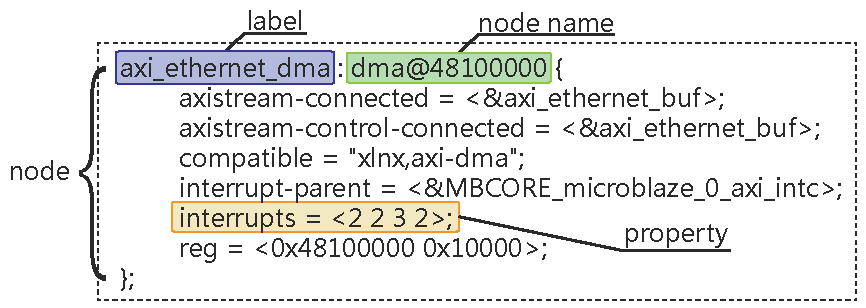
\includegraphics[width=0.75\textwidth]{impl/device-tree-example}
  \caption{DeviceTree示例}
  \label{fig:device-tree-example}
\end{figure}

由于PRM与逻辑域位于两个独立的系统,为了让PRM能够实现与逻辑域内存的数据传输,
在PRM中增加了一个DMA引擎,用于实现PRM内存与主系统内存之间的数据传输。
与带有DMA功能的I/O设备类似,该DMA引擎也需要增加标签寄存器,用于标记请求来源,
该寄存器同样通过$I^2C$总线连接到PRM。
PRM在启动DMA传输前,首先需要设置DMA的标签寄存器,将其设置为目标逻辑域的标签,
以保证数据被传输到正确的位置。
数据传输完成后,通过操作CoreCP相关的接口,启动逻辑域所在的处理器,
完成逻辑域操作系统启动。


\section{控制平面实现}
\label{chap:impl:cp}

本节在FPGA平台上实现了第\ref{chap:hwresman}章所介绍的控制平面微体系结构,
如图\ref{fig:generic-cp-schem}所示。
其中包括:$I^2C$接口模块、控制平面寄存器接口模块、
控制表地址解码模块和3个控制表。
其中$I^2C$接口模块与寄存器接口模块实现了控制平面网络接口模块的功能,
将通过控制平面网络发送的请求转换为对控制表的访问,
并通过控制表地址解码模块来访问3个控制表。
硬件数据平面更新的状态通过状态接口进入控制表,用于更新状态表;
状态表更新后会检查触发表,如果满足触发条件,则通过$I^2C$接口模块向PRM发送通知;
应用标签通过AXI总线的USER域传递到控制平面,用于查询参数表,并返回参数给数据平面。

\begin{figure}[htb]
  \centering
  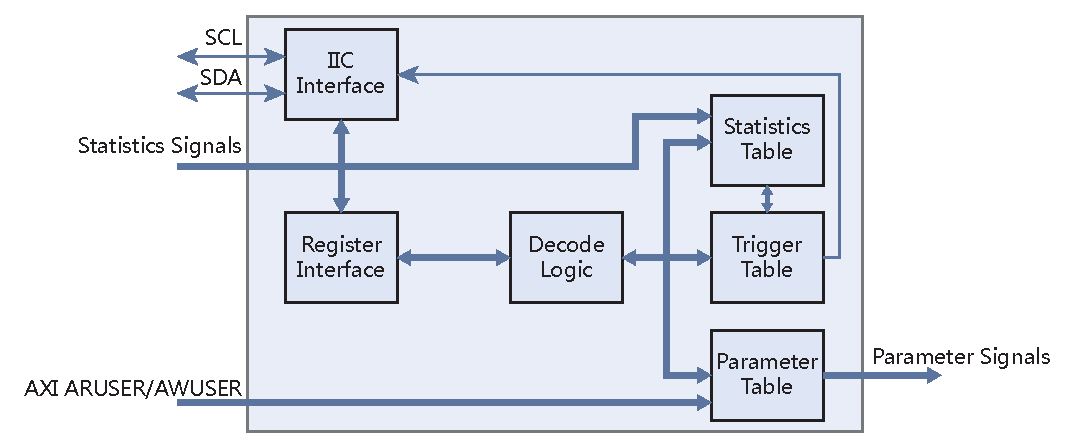
\includegraphics[width=0.80\textwidth]{impl/generic-cp-schem}
  \caption{控制平面结构框图}
  \label{fig:generic-cp-schem}
\end{figure}

Cache与内存控制器的控制平面实现与第\ref{chap:hwresman}章中介绍的基本相同,
本节不再赘述。
为了实现对处理器核的控制,以及标签寄存器的操作,
在原型系统中为处理器核也增加了控制平面。
该控制平面的参数表包含2项,分别用于设置标签寄存器、控制处理器核执行状态(启动、复位);
状态表记录了4个处理器核内部的统计信息,如IPC、TLB Miss、L1-I/D Miss等。

I/O控制平面的实现略复杂于以上3个控制平面,其主要功能有3个:
1)I/O地址映射;2)中断映射;3)DMA请求标记。
其中I/O地址映射的实现与内存控制器地址映射实现基本类似,
只是映射的目标地址范围有所差别。
内存控制器地址映射的目标地址范围是内存的物理地址范围,
在当前的I/O子系统实现中,其物理地址范围分配如表\ref{tab:pard-io-phyconfig}所示,
其中包括了2个以太网及其DMA控制器的寄存器范围、以及PCI-E控制寄存器与配置地址空间的范围,
I/O地址映射的目标地址范围只能在以上物理地址范围内。
I/O控制平面中增加了额外的配置表,
用于保存物理地址空间和中断(表\ref{tab:pard-io-phyconfig}),
在系统启动时,PRM通过I/O控制平面的配置表枚举系统中存在的设备,为后续的逻辑域设备分配做准备。
I/O控制平面的参数表使用``基址(base)''、``长度掩码(mask)''和``目标基址(rebase)''三个表项实现I/O地址映射,
使用``物理中断(phyintr)''、``目标中断(destintr)''两个表项实现中断映射。
用于DMA请求标记的标签寄存器是通过控制表中``标签(DSid)''进行控制。

\begin{table}[htb]
  \centering
  \begin{minipage}[t]{0.9\linewidth}
  \caption{I/O子系统物理地址空间与中断分配}
  \label{tab:pard-io-phyconfig}
    \begin{tabular*}{\linewidth}{ccll}
      \toprule[1.5pt]
      \textbf{地址范围} & \textbf{物理中断} & \textbf{硬件} & \textbf{用途} \\
      \midrule[1pt]
      0x48000000 - 0x4800FFFF & 1    & Ethernet \#0       & 控制寄存器    \\
      0x48100000 - 0x4810FFFF & 2, 3 & Ethernet DMA \#0   & DMA控制寄存器 \\
      0x48040000 - 0x4804FFFF & 4    & Ethernet \#1       & 控制寄存器    \\
      0x48110000 - 0x4811FFFF & 5, 6 & Ethernet DMA \#1   & DMA控制寄存器 \\
      0x60000000 - 0x6FFFFFFF & 10   & PCI-E Root Complex & 控制寄存器    \\
      0x70000000 - 0x7FFFFFFF & N/A  & PCI-E Root Complex & PCI-E地址空间 \\
      \bottomrule[1.5pt]
    \end{tabular*}\\[2pt]
  \end{minipage}
\end{table}


\subsection{分析}

虽然控制平面需要与请求的关键路径进行交互,
如Cache控制平面需要将路划分掩码参数送给Cache的LRU替换模块、
内存控制器控制平面需要将地址映射信息传递给MMU模块,
但控制平面并不会给请求处理带来额外的延迟。

对于Cache控制平面,第\ref{chap:hwresman}章中已经分析目前所使用的Cache都是基于流水线设计,
控制平面的操作可以隐藏在流水级当中,因此给请求带来额外的延迟开销。
对于内存控制器的地址映射(MMU)模块,
其控制平面参数表的数据通路上不存在任何锁存器,故可以在同一个周期内完成打标签和地址映射的功能,
图\ref{fig:migcp-latency-sim}所示的仿真结果也证明了内存控制器的MMU模块同样不会引入额外的延迟开销。

\begin{figure}[htb]
  \centering
  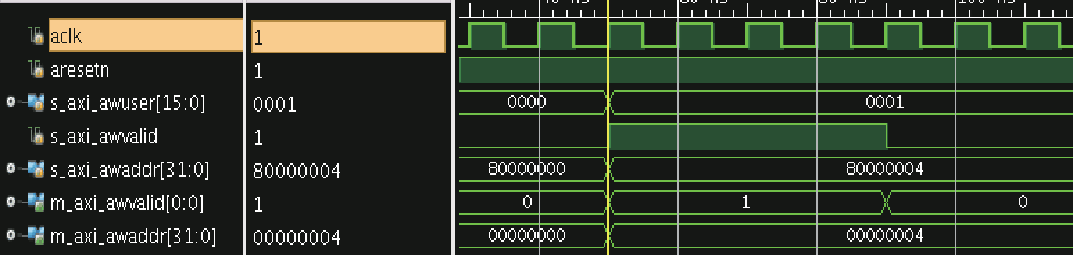
\includegraphics[width=0.9\textwidth]{impl/migcp-latency-sim}
  \caption[内存控制器控制平面地址映射功能仿真]{内存控制器控制平面地址映射功能仿真,结果表明没有对请求引入额外延迟}
  \label{fig:migcp-latency-sim}
\end{figure}


\section{数据平面实现}

为验证数据平面处理器的性能与资源开销,在内存控制器数据平面中增加数据平面处理器
(图\ref{fig:pard-fpga-routed}中migcp processors标记的区域),
通过执行软件代码的方式实现内存地址映射功能。
为简化实现,直接使用精简配置的MicroBlaze作为数据平面处理器,并对其进行以下改造:

\begin{enumerate}[leftmargin=2\parindent, nolistsep, label=\arabic*)]
  \item 将MicroBlaze配置为精简模式,去除所有与数据平面处理器无关的可选指令,
        如:硬件FPU、乘法器/除法器、扩展指令等;
        关闭MMU、Cache、中断异常等高级功能,只保留最基本的算术逻辑部分。
        通过精简配置,MicroBlaze系统的频率可以从133MHz提高到250MHz。
  \item 使用MicroBlaze提供的Stream Link接口作为数据平面处理器的请求接口。
        由于目前MicroBlaze的Stream Link接口是固定的32位AXIS接口,
        需要将多个Stream Link合并使用作为一个请求接口。
  \item MicroBlaze提供put/get指令实现对Stream Link的接口,
        通过合并多个put或get指令即可实现请求缓存指令rbput和rbget。
        如表\ref{tab:pard-dp-isa-impl}所示,``请求''类型的长度为12个字节,
        使用3个MicroBlaze通用寄存器(r10-r12)作为请求寄存器,
        使用get/put指令操作Stream Link接口fsl0,实现rbget和rbput的功能。
\end{enumerate}

\begin{table}[tb]
  \centering
  \begin{minipage}[t]{0.6\linewidth}
  \caption{请求缓存指令的MicroBlaze实现}
  \label{tab:pard-dp-isa-impl}
    \begin{tabular*}{\linewidth}{lp{0.5cm}lp{0.5cm}l}
      \toprule[1.5pt]
       & \multicolumn{2}{l}{\textbf{rbput}} & \multicolumn{2}{l}{\textbf{rbget}} \\ 
      \midrule[1pt]

      \multirow{8}{2cm}{\textbf{MicroBlaze指令实现}} & \multicolumn{2}{l}{rbput:}   & \multicolumn{2}{l}{rbget:} \\
                                                   &  & nget fsl0                 &  & nput fsl0               \\
                                                   &  & addc r3, r0, r0           &  & addc r3, r0, r0         \\
                                                   &  & bneq ret                  &  & bneq ret                \\
                                                   &  & get r10, fsl0             &  & put r10, fsl0           \\
                                                   &  & get r11, fsl1             &  & put r11, fsl1           \\
                                                   &  & get r12, fsg2             &  & put r12, fsl2           \\
                                                   & \multicolumn{2}{l}{ret:}     & \multicolumn{2}{l}{ret:}   \\
      \bottomrule[1.5pt]
    \end{tabular*}\\[2pt]
  \end{minipage}
\end{table}


\section{性能评价}

由于MicroBlaze的TLB中没有类似AccessBit的访问历史信息,
在当前的Linux内核实现中TLB替换策略使用clock算法,
造成应用在运行过程中频繁发生TLB miss与重填动作,
通过评估发现,有一半以上的时间都花费在kernel中执行TLB相关操作,
造成corecp和cachecp统计的IPC与命中率不准确。
为了得到准确的IPC与命中率信息,
需要将部分应用(429.mcf、cacheflush microbenchmark)移植到uboot环境下,
由于在uboot环境中由于并没有开启MMU,因此不会受到TLB的影响。
像memcached这样的应用,对操作系统的依赖很大,无法移植,
而这样的应用通常只关注其端到端的性能,因此TLB造成的性能差异可以忽略。


\subsection{区分化服务}

在PARD中使用逻辑域的抽象,可以为不同的逻辑域分配不同的资源,
本节将测试PARD如何为相同的应用分配不同的资源,以实现区分化服务的功能。
实验过程中同时运行两个配置完全相同的逻辑域,都包含一个处理器核和1GB内存,
两个逻辑域内运行相同的应用,通过Cache控制平面调整其缓存容量的分配,
验证PARD在末级缓存资源上区分化服务的效果。

图\ref{fig:diffserv-mcf-ipc-hitrate}给出了429.mcf的测试结果,
通过为两个逻辑域分配不同的缓存容量(4路和12路),
两个逻辑域内应用的总执行时间、以及缓存命中率存在明显的差别。
图\ref{fig:diffserv-memcached-rps}是使用memcached作为测试负载的结果,
分配到12路缓存的逻辑域,其运行过程中缓存命中率平均约为98.19\%,
而只分配到4路缓存的逻辑域,其缓存命中率只有77.19\%。
从最终memcached的性能来看,两者之间也存在了大约20\%的性能差别。

\begin{figure}[tb]
  \centering
  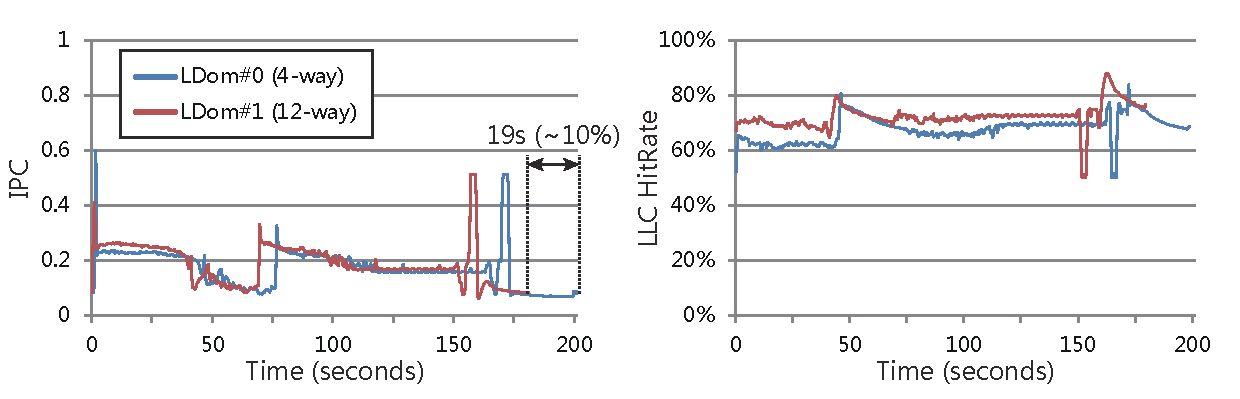
\includegraphics[width=\textwidth]{impl/diffserv-mcf-ipc-hitrate}
  \caption{区分化服务:429.mcf}
  \label{fig:diffserv-mcf-ipc-hitrate}
\end{figure}

\begin{figure}[tb]
\begin{minipage}[b]{0.48\textwidth}
  \centering
  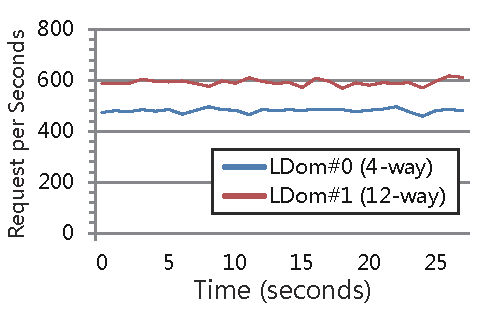
\includegraphics[width=\textwidth]{impl/diffserv-memcached-rps}
  \caption{区分化服务:memcached}
  \label{fig:diffserv-memcached-rps}
\end{minipage}\hfill
\begin{minipage}[b]{0.48\textwidth}
  \centering
  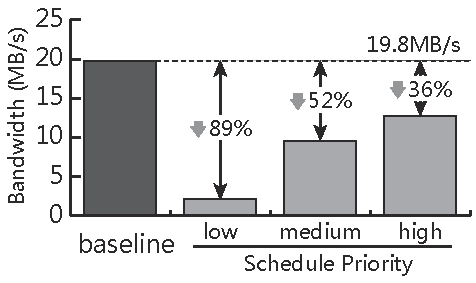
\includegraphics[width=\textwidth]{impl/diffserv-stream-generator}
  \caption{区分化服务:访存优先级}
  \label{fig:diffserv-stream-generator}
\end{minipage}
\end{figure}

为了评估在内存控制器控制平面提供的区分化服务功能,在本实验中关闭了Cache模块,
让处理器的访存请求直接发送到内存控制器。
使用stream benchmark\cite{stream}测试单个逻辑域的访存带宽为19.8MB/s,以此作为对比的基线。
在测试过程中发现,内存控制器所能提供的性能要远高于4个MicroBlaze处理器同时访存的需求,
为了进行本实验,需要对原型系统进行修改,使内存控制器发生资源竞争。
具体做法如下:将第4个处理器核更换为访存负载发生器,由它持续向内存控制器发送访存请求,
为了保证系统正确运行,该负载发生器只生成读请求,其余3个处理器核分别运行逻辑域,
并在其中使用stream benchmark发送读请求测试访存带宽。
在内存控制器控制平面为这3个逻辑域设置不同的优先级,同时为负载发生器设置为低优先级。
图\ref{fig:diffserv-stream-generator}给出了评测结果,
可以看到3个逻辑域的访存性能有明显的区分,相比于基线分别有89\%、52\%和36\%的带宽下降,
而负载发生器本身的访存带宽也从268MB/s下降到100MB/s。
目前内存控制器调度策略只实现了3个优先级,无法对每个逻辑域带宽进行精确控制,
后续可以对策略进行修改,以实现基于目标带宽的调度策略。


\subsection{性能隔离}

本节实验以Cache控制平面为例,验证PARD提供的性能隔离功能。
该实验同时启动4个逻辑域,在其中1个逻辑域内运行关键应用429.mcf或memcached,
另外3个逻辑域内运行干扰程序。

\begin{figure}[tb]
  \centering
  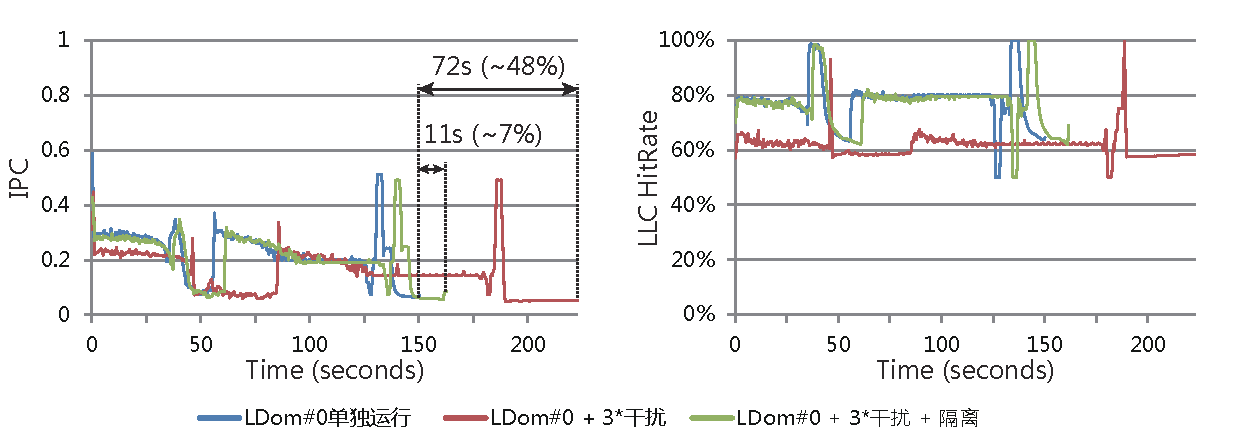
\includegraphics[width=\textwidth]{impl/isolation-mcf-ipc-hitrate}
  \caption{性能隔离:429.mcf}
  \label{fig:isolation-mcf-ipc-hitrate}
\end{figure}

\begin{figure}[tb]
  \centering
  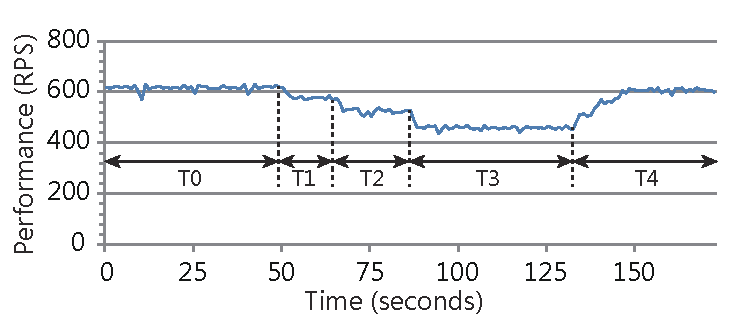
\includegraphics[width=0.6\textwidth]{impl/isolation-memcached}
  \caption{性能隔离:memcached}
  \label{fig:isolation-memcached}
\end{figure}

图\ref{fig:isolation-mcf-ipc-hitrate}给出了使用429.mcf负载的测试结果,
其中LDom\#0运行429.mcf,另外3个逻辑域运行干扰应用。
当LDom\#0单独运行时,它独占所有16路的Cache,执行时间大约为150秒;
与3个干扰应用同时运行时,执行时间延长到222秒,大约增加了48\%;
通过PARD提供的缓存隔离机制,将12路Cache分配给mcf,其性能基本恢复,
只增加了7\%的执行时间。

更换关键应用负载为memcached后,其测试结果如图\ref{fig:isolation-memcached}所示。
整个测试过程分为5个阶段:
T0阶段memcached单独运行,其性能大约为620RPS;
T1-T3阶段分别增加3个干扰应用,性能依次衰减到580RPS,520RPS和480RPS;
T4阶段通过Cache控制平面对缓存容量进行划分,将15路缓存分配给memcached所在逻辑域,
memcached的性能恢复到了600RPS左右。


\subsection{策略生效时间}
\label{chap:impl:trigger-latency}

本节实验测试通过``\emph{trigger$\Rightarrow$action}''机制实现缓存容量调整的效果及生效时间。
本实验使用memcached作为关键应用负载,实验过程与上节相同,在不同时间依次加入3个干扰应用。
与上节实验的区别在于,不需要手动调节容量划分,
而是使用``\emph{trigger$\Rightarrow$action}''机制进行自动调节。
具体方法如下:1)编写action动作脚本,在其中分配15路缓存给memcached所在逻辑域;
2)在Cache控制平面的触发表中增加触发条件``Cache缺失率超过30\%'',
并将其触发动作设置为1)中编写的动作脚本。

通过以上的配置修改后,在整个实验过程中,
增加的3个干扰应用并没有对memcached的性能造成任何的影响,
始终保持600RPS左右的性能。
分析整个``\emph{trigger$\Rightarrow$action}''的过程,
从触发条件满足到缓存容量划分策略生效总共经历了160ms的时间。
其中触发逻辑检测到条件满足到向PRM发送中断只需要2个时钟周期,即15ns(控制平面工作在133.33MHz频率);
PRM检测到中断发生需要1.6ms,响应动作(向参数表写入新策略)耗时约3ms;
除此之外的155ms都花费在了PRM执行动作脚本上,包括:
中断处理、进程创建,脚本执行等,由于FPGA平台和MicroBlaze核心性能的限制,
无法进一步提高PRM的频率与性能,如果使用真实芯片运行PRM,则可以大幅降低trigger响应时间。

%在PARD体系结构基于表的控制平面设计中,
%``Trigger$\Rightarrow$Action''机制的反馈时间可以主要分为Trigger事件检测、
%控制平面网络传送事件消息、PRM处理事件、以及控制平面网络传送Action的参数修改4个部分。
%其中第一阶段由控制表硬件逻辑完成,可以在有限的时钟周期内完成;
%第二和第四阶段由于需要使用控制平面网络传送数据,因此其响应时间与控制平面网络的速率相关,
%在我们目前的原型系统中,由于使用了$I^2C$总线作为控制平面网络,其最高速率为1Mbit/s,
%对于一个32bit的事件消息以及一组96bit的参数修改消息,至少需要128us完成数据传输,
%如果需要传输更多的消息则需要消耗更长的时间;
%第三阶段PRM处理中,需要经过控制平面驱动、内核、用户态3个层次进行处理,也需要消耗一定的时间。
%在采用可编程数据平面架构后,对Trigger事件的反馈调节代码可以直接在数据平面的固件代码中完成,
%消除了PARD原有设计中需要经过PRM进行统一处理的时间消耗,实现更快速的反馈响应。
%
%但数据平面处理器的引入也给性能造成影响,第\ref{chap:impl:dp-latency}节将对性能数据平面处理器的性能进行分析。


\subsection{数据平面处理器延迟分析}
\label{chap:impl:dp-latency}

%通过使用可编程处理器来替代硬件逻辑,可以极大增强设备的可编程能力,
%但由于处理器位于硬件请求处理的关键路径,我们需要对其性能与资源开销进行评估,
%以确保其不会对系统性能与开销造成严重的影响。
%本章以内存控制器的可编程数据平面为例,对其可编程数据平面的资源开销进行分析;
%并通过stream与memcached两种应用负载来评估其对系统性能的影响;
%最后我们分析了可编程数据平面架构对PARD体系结构中``Trigger=>Action''机制反馈时间的优化。

与硬件逻辑实现相比,可编程处理器在系统中引入了额外的开销,
本实验通过在内存控制器上增加可编程数据平面处理器,
验证可编程数据平面架构对系统延迟的影响。

系统延迟的大小与应用和固件功能相关,
因此固件代码选择与硬件实现完全相同的地址映射功能,
并使用stream和memcached对系统的延迟进行评估。
由于受到FPGA设备的限制,MicroBlaze软核处理器最高只能达到250MHz的频率,
因此实验中选择了100MHz/150MHz/200MHz/250MHz四种不同的频率对系统延迟进行了评估。

\textbf{访存带宽}\quad
在PARD的控制平面设计中,实现地址映射的控制表并没有引入额外的延迟开销,
其性能与直接访问内存控制器相同,受到MicroBlaze处理器性能的限制,
能够得到25.1MB/s的访存带宽(如图\ref{fig:pard-dp-stream}所示)。

由于地址映射功能只需要对请求地址进行操作,而无需对数据进行修改,
因此首先实现了一个简化版本的数据平面处理器(工作在100MHz频率),
该处理器只对地址请求进行处理,数据绕过处理器直接发送到内存控制器。
在使用该设计后测得的访存带宽是21.5MB/s,与非处理器实现相比并没有特别明显的下降。

为了使数据平面处理器对访存数据也能够进行操作,
将数据请求也发送到处理器进行处理,
在100MHz频率下测得的访存带宽出现了明显的下降,只有13MB/s。
进一步提高数据平面处理器的工作频率,带宽基本呈现线性上升,
在150MHz时能够得到15MB/s的访存带宽;
在200MHz时,访存带宽提高到了20MB/s;
而在250MHz时,访存带宽达到了22.5MB/s。
由于受到FPGA硬件的限制,无法实现更高频率的数据平面处理器,
但数据平面处理器的功能十分精简,如果使用ASIC工艺,可以得到更高的频率,
因此其处理器的性能不会成为系统的瓶颈。

\textbf{memcached性能}\quad
访存带宽只能作为系统性能的一个评估指标,系统运行时的实际开销要与应用相关联。
图\ref{fig:pard-dp-memcached}给出了memcached在同硬件配置下的性能变化,
与访存带宽的结果类似,memcached的性能与数据平面处理器频率相关,
当工作在100MHz频率时,只能得到568RPS的性能,
但如果处理器频率提升到250MHz,其性能(618RPS)与使用控制表的方案(628RPS)基本接近。

\begin{figure}[tb]
\begin{minipage}{0.48\textwidth}
  \centering
  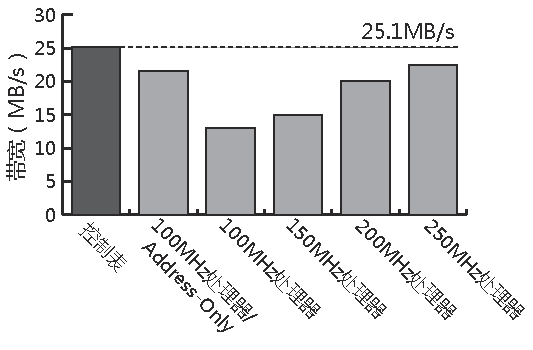
\includegraphics[width=\textwidth]{impl/pard-dp-stream}
  \caption{访存带宽对比}
  \label{fig:pard-dp-stream}
\end{minipage}\hfill
\begin{minipage}{0.48\textwidth}
  \centering
  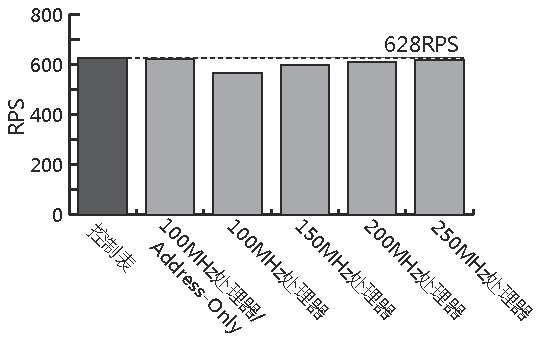
\includegraphics[width=\textwidth]{impl/pard-dp-memcached}
  \caption{memcached性能对比}
  \label{fig:pard-dp-memcached}
\end{minipage}
\end{figure}


\subsection{资源开销评价}

PARD的资源开销主要体现在3个方面,分别是:
用于标签传播的资源开销、
控制平面的资源开销、
数据平面的资源开销。
本节将分别对这3个方面的开销进行评估。

\subsubsection{标签传播资源开销}

PARD的标签机制会在数据通路上产生额外的资源开销,对应到FPGA原型系统,
该开销主要体现在系统中AXI CrossBar和Cache两部分,
本节将对标签机制在这两部分中产生的资源开销进行评估。
为了便于比较,CrossBar和Cache都配置为9个AXI Slave端口和1个AXI Master端口,
同时评估了4种不同配置下(无标签、8位标签、16位标签和32位标签)的资源开销,
结果如图\ref{fig:xbar-dsid-overhead}和图\ref{fig:cache-dsid-overhead}所示。
为了方便对比,图\ref{fig:cache-dsid-overhead}中Block RAM的资源为放大10倍后的结果,
其原始数据分别为153、157、161和169。

对于CrossBar,不同长度的标签并没有带来特别大的资源占用,
相比无标签情况,16位标签额外增加了6.86\%的Slice LUT资源以及3.91\%的Slice Register资源。
对于Cache,由于需要在TagArray中保存Owner-DSid,
并且在逻辑中增加DSid的比较逻辑,其资源占用比CrossBar有所增加,
同样相比无标签情况,16位标签额外增加了11.97\%的Slice LUT资源、
24.36\%的Slice Register资源、以及5.23\%的Block RAM资源。

\begin{figure}[tb]
\begin{minipage}{0.48\textwidth}
  \centering
  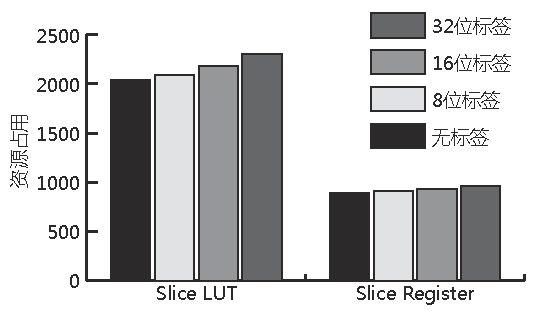
\includegraphics[width=\textwidth]{impl/xbar-dsid-overhead}
  \caption{CrossBar标签开销}
  \label{fig:xbar-dsid-overhead}
\end{minipage}\hfill
\begin{minipage}{0.48\textwidth}
  \centering
  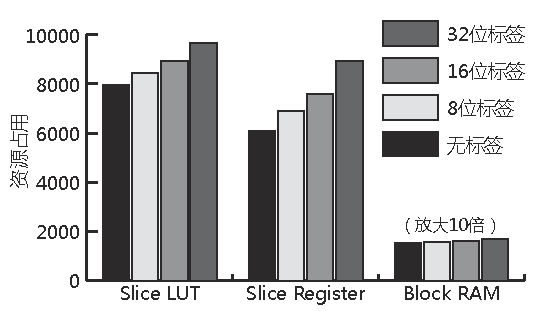
\includegraphics[width=\textwidth]{impl/cache-dsid-overhead}
  \caption{Cache标签开销}
  \label{fig:cache-dsid-overhead}
\end{minipage}
\end{figure}


\subsubsection{控制平面资源开销}

控制平面的资源开销主要体现在表存储、触发逻辑两方面,
由于控制表使用了CAM结构,无法使用FPGA中的BRAM资源实现表存储,
因此需要消耗一定量的LUT和Register资源,不过与全系统占用的资源总量相比,
这部分的资源开销并不大。
4个控制平面总计占用了全系统LUT用量的3.66\%和Register用量的4.52\%,
根据控制表的功能、表项设计的不同,不同控制平面的资源开销略有不同,
具体的资源占用如表\ref{tab:pard-cp-resource}所示。

\begin{table}[htb]
  \centering
  \caption{控制平面资源占用情况(xc7vx690t设备)}
  \label{tab:pard-cp-resource}
  \begin{tabular*}{\linewidth}{rcccccccc}
    \toprule[1.5pt]
          & \multicolumn{4}{c}{\textbf{Slice LUT}}  & \multicolumn{4}{c}{\textbf{Slice Register}} \\
          & 参数表 & 状态表 & 触发表 & 小计(\%)   & 参数表 & 状态表 & 触发表 & 小计(\%)       \\
    \midrule[1pt]
     Core &     94 &    806 &    202 & 1102(0.90\%) &    104 &   1296 &    109 & 1509(1.10\%)      \\
    Cache &     51 &   1030 &    203 & 1284(1.04\%) &     96 &   1874 &    109 & 2079(1.51\%)      \\
      Mem &    291 &    487 &    169 &  947(0.77\%) &    320 &    768 &    109 & 1197(0.87\%)      \\
      I/O &    508 &    487 &    169 & 1164(0.95\%) &    560 &    768 &    109 & 1437(1.04\%)      \\
    \hline
   全系统 & \multicolumn{4}{c}{122,960}             & \multicolumn{4}{c}{137,797}                  \\
    \bottomrule[1.5pt]
  \end{tabular*}\\[2pt]
\end{table}

\subsubsection{数据平面资源开销}

可编程数据平面的资源开销主要在处理器逻辑及其使用的scratchpad memory两个方面。
在通过配置精简后,MicroBlaze处理器所占用的资源量大大减少,
其Slice(LUT和Register)占用只有完整配置的50\%左右,
scratchpad memory的容量由固件代码的大小决定,
当前的实现中将其配置为32KB,在FPGA中占用了8个RAMB36资源。
原型系统中主要的硬件部件与可编程数据平面占用的FPGA资源如表\ref{tab:pard-dp-resource}所示。
可编程数据平面在只占用有限的FPGA资源下,为硬件增加了更为灵活的可编程能力。

\begin{table}[htb]
  \centering
  \begin{minipage}[t]{0.9\linewidth}
  \caption{数据平面处理器、共享缓存与内存控制器资源占用情况(xc7vx690t设备)}
  \label{tab:pard-dp-resource}
    \begin{tabular*}{\linewidth}{cccc}
      \toprule[1.5pt]
      \textbf{组件} & \textbf{Slice LUT} & \textbf{Slice Register} & \textbf{Block RAM(RAMB36)} \\
      \midrule[1pt]
      16-way/512KB共享缓存    &  7590       &  5664            &  161               \\
      内存控制器              &  13471      &  10562           &  1                 \\
      完整配置的MicroBlaze核  &  4896       &  8526            &  12                \\
      \hline
      数据平面处理器          &  1433       &  5524            &  8                 \\
      \bottomrule[1.5pt]
    \end{tabular*}\\[2pt]
  \end{minipage}
\end{table}


\section{小结}

本章对前述章节中资源管理可编程体系结构PARD的设计进行了原型系统实现,包括模拟器与FPGA原型两部分。
主要对FPGA原型系统中可编程控制平面和可编程数据平面的功能进行验证,并评估其性能与资源开销。
实验结果表明,该原型系统能够实现本文所提出的全部功能,包括:
1)无软件Hypervisor支持的全硬件虚拟化;2)应用区分化服务;3)性能隔离。
PARD体系结构的扩展并不会对系统性能造成影响,也不会增加过多的资源开销;
在此基础上,能够实现应用的区分化服务、细粒度的资源管理、以及性能隔离,
能够适应于数据中心这种复杂多变的共享场景中,实现应用服务质量与资源利用率的平衡。


\begin{figure}[htb]
  \centering
  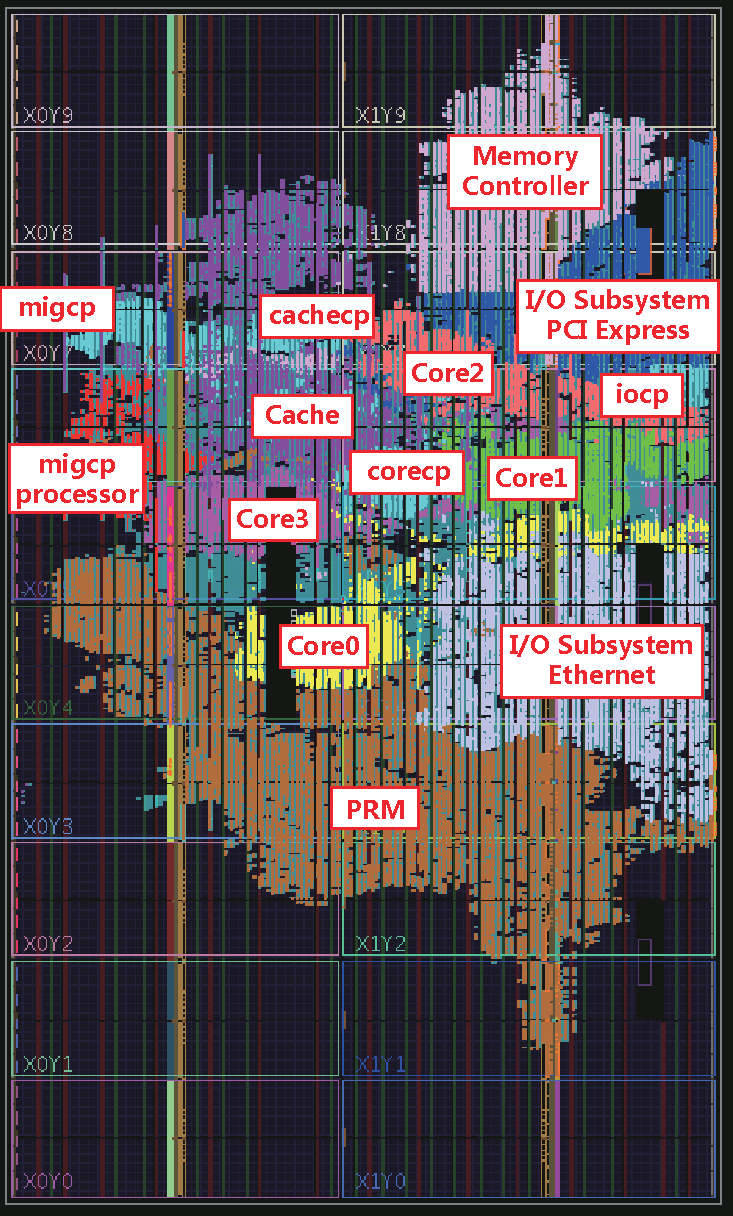
\includegraphics[width=0.8\textwidth]{impl/pard-fpga-routed}
  \caption{PARD原型系统布局布线结果}
  \label{fig:pard-fpga-routed}
\end{figure}
